\documentclass[12pt]{article}

%\usepackage{mathptm}  
\usepackage{a4}
\usepackage{hyperref}
\usepackage{color}
\usepackage{graphicx}
\usepackage{fancyhdr}
\usepackage{multicol}
\usepackage{amstext}
\usepackage{amsmath}
%\usepackage{fullpage}
%\usepackage{parskip}
\usepackage[colon]{natbib}
%\usepackage{rotating}
\usepackage{pdflscape}
\usepackage{longtable}
\usepackage{caption}
\usepackage{subcaption}
%\usepackage[nomarkers,figuresonly]{endfloat}
\usepackage{amsfonts}
\usepackage{pifont}
\usepackage{authblk}
\usepackage{epstopdf}
\usepackage{multirow}
\usepackage{amsfonts}

\textwidth 160mm
\textheight 235mm
\oddsidemargin 0mm
\topmargin -15mm
\baselineskip 13pt
\parskip 1pc
\parindent 0pc

\pagestyle{fancy}
\cfoot{\thepage}

\renewcommand{\headrulewidth}{0.2pt}
\renewcommand{\footrulewidth}{0.2pt}

\newcommand\Bo{\mbox{\textit{Bo}}}  % Bond number
\newcommand\Ca{\mbox{\textit{Ca}}} %Capillary number

\definecolor{darkred}{rgb}{0.80,0.00,0.05}
\definecolor{blue}{rgb}{0.00,0.00,0.95}
\definecolor{darkgreen}{rgb}{0.00,0.60,0.0}
\definecolor{gray}{rgb}{0.95,0.9,0.9}

\usepackage{listings}
\lstset{language=C++}
\lstset{backgroundcolor=\color{gray}}
\lstset{breaklines=true}
\lstset{basicstyle=\ttfamily\small}
\lstset{showstringspaces=false}
\lstset{keywordstyle=\color{blue}\bfseries}
\lstset{commentstyle=\ttfamily\small\color{darkgreen}}
\lstset{identifierstyle=\color{darkred}\bfseries}
\lstset{numbers=left,numberstyle=\tiny}
\lstset{columns=fixed,basewidth=0.45em}

\DeclareMathOperator\erf{erf}

\linespread{1.5}

\begin{document}
\thispagestyle{empty}

\title{Low Reynolds number gravitational settling of a sphere through a fluid-fluid interface: Modelling using a boundary integral method}

\author[1]{Paul Jarvis\footnote{Corresponding author:paul.jarvis@bristol.co.uk}}
\author[1]{Jon Blundy}
\author[1]{Katharine Cashman}
\author[1,2]{Herbert E Huppert}
\author[1]{Heidy Mader}
\affil[1]{\small School of Earth Sciences, University of Bristol, Wills Memorial Building, Queens Road, Bristol, BS8 1RJ, UK}
\affil[2]{\small Department of Applied Mathematics and Theoretical Physics, University of Cambridge, Wilberforce Road, Cambridge, CB3 0WA, UK}
\date{}
% NOTE: A full address must be provided: department, university/institution, town/city, zipcode/postcode, country.


\maketitle

\begin{abstract}


\end{abstract}


\section{Introduction}


\section{Theoretical Development}

  \begin{figure}
    $$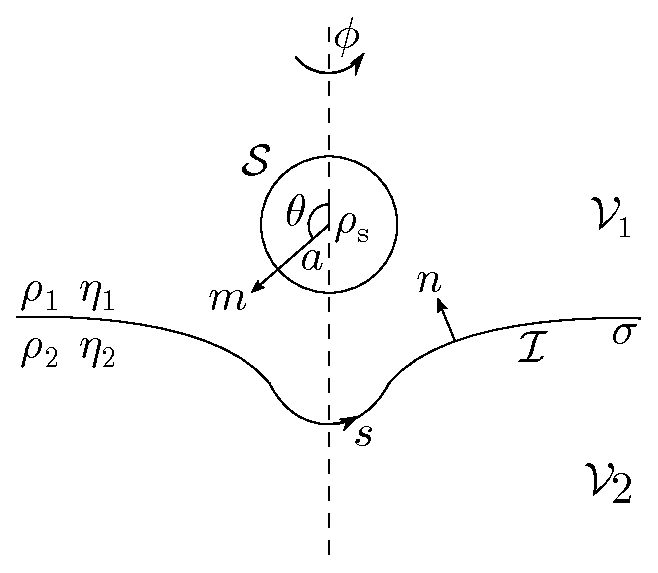
\includegraphics[width=\textwidth]{formulation.eps}$$
    \caption{Diagrammatic representation of the system. See table (NEED TO MAKE SYMBOL TABLE) for definition of symbols. \label{fig:params}}
  \end{figure}



%\bibliographystyle{plainnat}

%\bibliography{fluids}


\end{document}